\documentclass{article}[11pt]

\usepackage{amsmath}
\usepackage{amssymb}
\usepackage{nicefrac}

\usepackage{pdflscape}

\usepackage{upgreek}

\usepackage{bashful}

% No intendation
\setlength\parindent{0pt}

\usepackage{hyperref}

\usepackage{siunitx}
\sisetup{
  per-mode=fraction,
  fraction-function=\tfrac
}

\usepackage{listings}
  \lstset{
    basicstyle=\ttfamily,
    escapeinside=||,
    xleftmargin=1cm
  }

\usepackage{float}

\usepackage{longtable}

\usepackage{multirow}

\usepackage{tikz}
  \usetikzlibrary{patterns}
  \usetikzlibrary{arrows.meta}
  \usetikzlibrary{shapes.misc}
  \usetikzlibrary{calc}

\usepackage{pgfplots}

\usepackage{cleveref}
\crefmultiformat{equation}{(#2#1#3)}{ and~(#2#1#3)}{, (#2#1#3)}{ and~(#2#1#3)}


\usepackage{acronym}
\usepackage[acronym,nonumberlist]{glossaries}
\glsdisablehyper
\makeglossaries
\newacronym{spice}{SPICE}{Simulation Program with Integrated Circuit Emphasis}
\newacronym{lef}{LEF}{Library Exchange Format}
\newacronym{dft}{DFT}{Discrete Fourier Transform}
\newacronym{dtft}{DTFT}{Discrete-Time Fourier Transform}
\newacronym{fft}{FFT}{Fast Fourier Transform}
\newacronym{mosfet}{MOSFET}{Metal–Oxide–Semiconductor Field-Effect Transistor}
\newacronym{clm}{CLM}{Channel Length Modulation}
\newacronym{de}{DE}{differential equation}
\newacronym{soi}{SOI}{silicon-on-insulator}
\newacronym{ldo}{LDO}{low-dropout regulator}
\newacronym{ota}{OTA}{operational-transconductance amplifier}
\newacronym{ofa}{OFA}{operational-floating amplifier}

% literature
\usepackage[ backend=biber
           , isbn=true
           , sorting=none
           , style=ieee
           ]{biblatex}
\addbibresource{./../../literature.bib}

% definitions
\def \whatis       {Notes}
\def \title        {Fuubar}

\def \author       {Matthias Schweikardt}

\def \authorMail   {mschweikardt@posteo.de}

\def \authorGithub {mschweikardt}

\def \license      {CC BY-SA 4.0}
\def \licenseUrl   {https://creativecommons.org/licenses/by-sa/4.0/}

\def \date         {nodate}

\def \pdfurl       {https://mschweikardt.github.io/ee-notes/%
\bash[stdout]
IFS=/ 
var=($PWD)
echo ${var[-1]}
\END%
.pdf
}
\def \srcurl       {srcurl}


% Customize footer and header of document
\usepackage{fancyhdr}

% Access last page number
\usepackage{lastpage}

% Access last page number
\usepackage[thinc]{esdiff}

% Physics
\usepackage{physics}

% Comment environment
\usepackage{comment}

% Subcaptions
\usepackage{subcaption}

% Thicker lines in tables
\usepackage{booktabs}

% Indentation in footnote
\makeatletter
\renewcommand\@makefntext[1]{\leftskip=2em\hskip-0.5em\@makefnmark#1}
\makeatother         

% qty with the siunitx definition
\AtBeginDocument{\RenewCommandCopy\qty\SI}

% TikZ compatibility
\pgfplotsset{compat=1.18}


\makeatletter
\pgfmathdeclarefunction{myatan2}{2}{%
\begingroup%
  \pgfmathfloattofixed{#1}\edef\tempa{\pgfmathresult}%
  \pgfmathfloattofixed{#2}%
  \pgfkeys{pgf/fpu=false}%
  \pgfmathparse{atan2(\tempa,\pgfmathresult)}\pgfkeys{/pgf/fpu}%
  \pgfmathfloatparsenumber{\pgfmathresult}%
  \pgfmath@smuggleone\pgfmathresult%
\endgroup
}
\makeatother

\usepackage{tabularx}
% usepackages
\usepackage[ a4paper
           , textwidth  = 16.0cm
           , textheight = 25.0cm
           , headsep    =  0.25cm
           , voffset    =  0.3cm
           , footskip   =  1.25cm
           ]{geometry}

% Section and subsection enumeration
\renewcommand{\thesection}{\Roman{section}.} 
\renewcommand{\thesubsection}{\thesection\Alph{subsection}}

\usepackage{titlesec}
\titleformat{\section}
  {\normalfont\Large\bfseries}{\thesection}{0.2em}{}
\titleformat{\subsection}
  {\normalfont\large\bfseries}{\thesubsection}{0.2em}{}


% Defince title of document
\newcommand{\notetitle}{
  \begingroup
  \hypersetup{hidelinks}
  \thispagestyle{notefirst}
  \begin{center}
  \rule{\textwidth}{1pt}\\
  \medskip
  {\it \whatis}\\
  \bigskip
  {\LARGE \textbf{\title}}\\
  \medskip
  {\small \author}\\
  \rule{\textwidth}{0.5pt}\\
  {\small
    \begin{minipage}[t]{0.5\textwidth}
      \begin{tabular}[t]{ p{2.25cm} p{5.75cm}}
        Mail: & \href{mailto:\authorMail}{\tt{\authorMail}} \\
        Github: & \href{https://github.com/\authorGithub}{\tt{\authorGithub}} \\
      \end{tabular}
    \end{minipage}%
    %
    \begin{minipage}[t]{0.5\textwidth}
      \begin{tabular}[t]{ p{2.25cm} p{5.75cm} }
        Date: & \date  \\
        License: & \href{\licenseUrl}{\license}
      \end{tabular}
    \end{minipage}
  }%
  {\small
    \begin{minipage}[t]{\textwidth}
      \begin{tabular}[t]{ p{2.25cm} p{12cm}}
        Latest PDF: & \href{\pdfurl}{\tt{\pdfurl}} \\
        Latest Source: & \href{\srcurl}{\tt{\srcurl}}
      \end{tabular}
    \end{minipage}%
  }
  \bigskip
  \rule{\textwidth}{1pt}
  \end{center}
  \endgroup
}

% Header and footer on first page
\fancypagestyle{notefirst}{
  \fancyhf{}
  \renewcommand{\headrulewidth}{0pt}
  \renewcommand{\footrulewidth}{0pt}

  \fancyfoot[C]{\thepage/\pageref*{LastPage}}
}

% Header and footer on 2nd-last page
\fancypagestyle{noterest}{
  \fancyhf{}
  \renewcommand{\headrulewidth}{0.5pt}
  \renewcommand{\footrulewidth}{0.0pt}

  \fancyhead[L]{\author}
  \fancyhead[C]{\title}
  \fancyhead[R]{\date}

  \fancyfoot[C]{\thepage/\pageref*{LastPage}}
}
\pagestyle{noterest}

\usepackage{amsmath}
\usepackage{amssymb}
\usepackage{nicefrac}

\usepackage{pdflscape}

\usepackage{upgreek}

\usepackage{bashful}

% No intendation
\setlength\parindent{0pt}

\usepackage{hyperref}

\usepackage{siunitx}
\sisetup{
  per-mode=fraction,
  fraction-function=\tfrac
}

\usepackage{listings}
  \lstset{
    basicstyle=\ttfamily,
    escapeinside=||,
    xleftmargin=1cm
  }

\usepackage{float}

\usepackage{longtable}

\usepackage{multirow}

\usepackage{tikz}
  \usetikzlibrary{patterns}
  \usetikzlibrary{arrows.meta}
  \usetikzlibrary{shapes.misc}
  \usetikzlibrary{calc}

\usepackage{pgfplots}

\usepackage{cleveref}
\crefmultiformat{equation}{(#2#1#3)}{ and~(#2#1#3)}{, (#2#1#3)}{ and~(#2#1#3)}


\usepackage{acronym}
\usepackage[acronym,nonumberlist]{glossaries}
\glsdisablehyper
\makeglossaries
\newacronym{spice}{SPICE}{Simulation Program with Integrated Circuit Emphasis}
\newacronym{lef}{LEF}{Library Exchange Format}
\newacronym{dft}{DFT}{Discrete Fourier Transform}
\newacronym{dtft}{DTFT}{Discrete-Time Fourier Transform}
\newacronym{fft}{FFT}{Fast Fourier Transform}
\newacronym{mosfet}{MOSFET}{Metal–Oxide–Semiconductor Field-Effect Transistor}
\newacronym{clm}{CLM}{Channel Length Modulation}
\newacronym{de}{DE}{differential equation}
\newacronym{soi}{SOI}{silicon-on-insulator}
\newacronym{ldo}{LDO}{low-dropout regulator}
\newacronym{ota}{OTA}{operational-transconductance amplifier}
\newacronym{ofa}{OFA}{operational-floating amplifier}

% literature
\usepackage[ backend=biber
           , isbn=true
           , sorting=none
           , style=ieee
           ]{biblatex}
\addbibresource{./../../literature.bib}

% definitions
\def \whatis       {Notes}
\def \title        {Fuubar}

\def \author       {Matthias Schweikardt}

\def \authorMail   {mschweikardt@posteo.de}

\def \authorGithub {mschweikardt}

\def \license      {CC BY-SA 4.0}
\def \licenseUrl   {https://creativecommons.org/licenses/by-sa/4.0/}

\def \date         {nodate}

\def \pdfurl       {https://mschweikardt.github.io/ee-notes/%
\bash[stdout]
IFS=/ 
var=($PWD)
echo ${var[-1]}
\END%
.pdf
}
\def \srcurl       {srcurl}


% Customize footer and header of document
\usepackage{fancyhdr}

% Access last page number
\usepackage{lastpage}

% Access last page number
\usepackage[thinc]{esdiff}

% Physics
\usepackage{physics}

% Comment environment
\usepackage{comment}

% Subcaptions
\usepackage{subcaption}

% Thicker lines in tables
\usepackage{booktabs}

% Indentation in footnote
\makeatletter
\renewcommand\@makefntext[1]{\leftskip=2em\hskip-0.5em\@makefnmark#1}
\makeatother         

% qty with the siunitx definition
\AtBeginDocument{\RenewCommandCopy\qty\SI}

% TikZ compatibility
\pgfplotsset{compat=1.18}


\makeatletter
\pgfmathdeclarefunction{myatan2}{2}{%
\begingroup%
  \pgfmathfloattofixed{#1}\edef\tempa{\pgfmathresult}%
  \pgfmathfloattofixed{#2}%
  \pgfkeys{pgf/fpu=false}%
  \pgfmathparse{atan2(\tempa,\pgfmathresult)}\pgfkeys{/pgf/fpu}%
  \pgfmathfloatparsenumber{\pgfmathresult}%
  \pgfmath@smuggleone\pgfmathresult%
\endgroup
}
\makeatother

\usepackage{tabularx}


\def \title  {Switches}
\def \date   {June 8, 2025}

\def \pdfurl {https://mschweikardt.github.io/ee-notes/switches.pdf}
\def \srcurl {https://github.com/mschweikardt/ee-notes/tree/main/notes/switches}

\usepackage[scale=5]{draftwatermark}

\begin{document}

\notetitle

\section{NMOS-Switch}




\begin{circuitikz}

  \node[nmos, rotate=90](m1) at (0,0) {};

  \draw (m1.gate) to[short,-o] ++ (0,-0.25) coordinate (s)
                  to[V,o-,v=$v_{\mathrm{S}}(t)$] ++ (0,-2) coordinate (gnd); 
  \node[anchor=east] at (s) {S};

  \draw (m1.drain) to [short,-o] ++ (-0.5,0) coordinate (inp)
                   to [short,-,i<_=$i(t)$] ++ (-1.25,0) coordinate (vinp)
                   to [V,-,v=$V_{\mathrm{in}}$] (vinp|-gnd)  coordinate (vinn)
                   to [short,-o] (vinn-|inp) coordinate (inn)
                   to [short,-*] (gnd);

  \draw (m1.source) to [short,-o] ++ (0.75,0) coordinate (outp)
                    to [short,-] ++ (1.25,0) coordinate (voutp)
                    to [C,l_=$C_{\mathrm{L}}$,v^=$v_{\mathrm{O}}(t)$] 
                      (voutp|-gnd)  coordinate (voutn)
                    to [short,-o] (voutn-|outp) coordinate (outn)
                    to [short,-*] (gnd);

  \node[anchor=south] at (inp) {I};
  \node[anchor=south] at (outp) {O};

  \node[ground] at (gnd) {};
\end{circuitikz} 

\begin{table}[H]
\centering
\caption{Events of the NMOS-Switch}
\begin{tabular}{cccccccc}
\toprule
\multirow{2}{*}{\textit{Event}} & \multirow{2}{*}{\textit{Operation}} & \multicolumn{2}{c}{$V_{\mathrm{in}}$}                                 & \multicolumn{2}{c}{$V_{0}$}                                           & \multirow{2}{*}{$i(t)$}   & \multirow{2}{*}{$v_{\mathrm{O}}(t_{\mathrm{S}})$}  \\ 
~                               & ~                                   & min                               & max                               & min                               & max                               & ~                         & ~                                                  \\ \midrule
A                               & charging                            & 0                                 & $V_{\mathrm{DD}}-V_{\mathrm{TH}}$ & 0                                 & $V_{\mathrm{in}}$                 & $\geq0$                   & $V_{\mathrm{in}}$                                  \\ 
B                               & charging                            & $V_{\mathrm{DD}}-V_{\mathrm{TH}}$ & $V_{\mathrm{DD}}$                 & 0                                 & $V_{\mathrm{DD}}-V_{\mathrm{TH}}$ & $\geq0$                   & $V_{\mathrm{in}}-V_{\mathrm{TH}}$                  \\ 
C                               & -                                   & $V_{\mathrm{DD}}-V_{\mathrm{TH}}$ & $V_{\mathrm{DD}}$                 & $V_{\mathrm{DD}}-V_{\mathrm{TH}}$ & $V_{\mathrm{in}}$                 & $=0$                      & $V_{0}$                                            \\ 
D                               & -                                   & $V_{\mathrm{DD}}-V_{\mathrm{TH}}$ & $V_{\mathrm{DD}}$                 & $V_{\mathrm{in}}$                 & $V_{\mathrm{DD}}$                 & $=0$                      & $V_{0}$                                            \\ 
E                               & discharging                         & 0                                 & $V_{\mathrm{DD}}-V_{\mathrm{TH}}$ & $V_{\mathrm{DD}}-V_{\mathrm{TH}}$ & $V_{\mathrm{DD}}$                 & $\leq0$                   & $V_{\mathrm{in}}$                                  \\ 
F                               & discharging                         & 0                                 & $V_{\mathrm{DD}}-V_{\mathrm{TH}}$ & $V_{\mathrm{in}}$                 & $V_{\mathrm{DD}}-V_{\mathrm{TH}}$ & $\leq0$                   & $V_{\mathrm{in}}$                                  \\ \toprule
\end{tabular}
\label{tab:os}
\end{table}

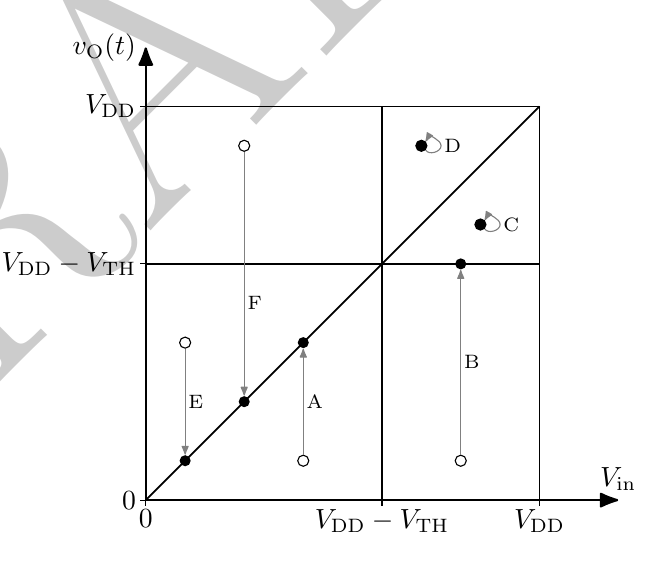
\begin{tikzpicture}
  \useasboundingbox (-1.5,-0.5) rectangle (6.25,6);

  \draw[semithick] (0,0) rectangle (5,5);
  \draw[semithick] (3,0) rectangle (5,3);
  \draw[semithick] (0,0) -- (5,5);
  \draw[semithick] (0,3) rectangle (3,5);

  %\node[rotate=90] at (0.75,2.5) {off};
  %\node[] at (4.0,0.75) {ohmic};
  %\node[] at (3.25,3.5) {saturation};

  \node[anchor=north] at (0,0) {0};
  \draw[thin] (0,0) -- (0,-0.075);
  \node[anchor=east] at (0,0) {0};
  \draw[thin] (0,0) -- (-0.075,0);

  \node[anchor=north] at (3,0) {$V_{\mathrm{DD}}-V_{\mathrm{TH}}$};
  \draw[thin] (3,0) -- (3,-0.075);

  \node[anchor=north] at (5.0,0) {$V_{\mathrm{DD}}$};
  \draw[thin] (5.0,0) -- (5.0,-0.075);

  \node[anchor=east] at (0,5) {$V_{\mathrm{DD}}$};
  \draw[thin] (0,5) -- (-0.075,5);

  \node[anchor=east] at (0,3) {$V_{\mathrm{DD}}-V_{\mathrm{TH}}$};
  \draw[thin] (0,3) -- (-0.075,3);

  \draw[{Latex[round,scale=1.2]}-{Latex[round,scale=1.2]},thick] 
    (0,5.75) -- (0,0) -- (6,0);

  \node[anchor=south] at (6,0) {$V_{\mathrm{in}}$};
  \node[anchor=east] at (0,5.75) {$v_{\mathrm{O}}(t)$};

  \node[circle,draw,color=black,fill=white,inner sep=0pt,minimum size=4pt] (a1) at (2,0.5) {};
  \node[circle,fill=black,inner sep=0pt,minimum size=4pt] (a2) at (2,2) {};
  \draw[-{Latex[round,scale=0.8]},gray] (a1) -- (a2) 
    node[midway,font=\scriptsize,right,inner sep=1pt,black] {A};

  \node[circle,draw,color=black,fill=white,inner sep=0pt,minimum size=4pt] (b1) at (4,0.5) {};
  \node[circle,fill=black,inner sep=0pt,minimum size=4pt] (b2) at (4,3) {};
  \draw[-{Latex[round,scale=0.8]},gray] (b1) -- (b2) 
    node[midway,font=\scriptsize,right,inner sep=1pt,black] {B};

  \node[circle,draw,color=black,fill=white,inner sep=0pt,minimum size=4pt] (c1) at (4.25,3.5) {};
  \node[circle,fill=black,inner sep=0pt,minimum size=4pt] (c2) at (4.25,3.5) {};
  \draw[-{Latex[round,scale=0.8]},gray] (c1.south east) to [out=-60,in=-90] (4.5,3.5)
        node[right,font=\scriptsize,right,inner sep=1pt,black] {C}
        to [out=90,in=60] (c2.north east);

  \node[circle,draw,color=black,fill=white,inner sep=0pt,minimum size=4pt] (d1) at (3.5,4.5) {};
  \node[circle,fill=black,inner sep=0pt,minimum size=4pt] (d2) at (3.5,4.5) {};
  \draw[-{Latex[round,scale=0.8]},gray] (d1.south east) to [out=-60,in=-90] (3.75,4.5)
        node[right,font=\scriptsize,right,inner sep=1pt,black] {D}
        to [out=90,in=60] (d2.north east);

  \node[circle,draw,color=black,fill=white,inner sep=0pt,minimum size=4pt] (f1) at (1.25,4.5) {};
  \node[circle,fill=black,inner sep=0pt,minimum size=4pt] (f2) at (1.25,1.25) {};
  \draw[-{Latex[round,scale=0.8]},gray] (f1) -- (f2) 
    node[midway,font=\scriptsize,right,inner sep=1pt,black,pos=0.62] {F};

  \node[circle,draw,color=black,fill=white,inner sep=0pt,minimum size=4pt] (e1) at (0.5,2) {};
  \node[circle,fill=black,inner sep=0pt,minimum size=4pt] (e2) at (0.5,0.5) {};
  \draw[-{Latex[round,scale=0.8]},gray] (e1) -- (e2) 
    node[midway,font=\scriptsize,right,inner sep=1pt,black] {E};
\end{tikzpicture}

\begin{itemize}
\item Switch
\begin{equation}
v_{\mathrm{S}}(t) =
\begin{cases}
0               & \mathrm{when} \ t < 0    \\
V_{\mathrm{DD}} & \mathrm{when} \ t \geq 0 \\
\end{cases}.
\end{equation}
\item $v_{\mathrm{O}}(0) = V_0$
\end{itemize}



\paragraph{Event A}

\begin{itemize}
\item I = Drain, O=Source
\item $v_{\mathrm{GS}}(t) = V_{\mathrm{DD}}-v_{\mathrm{O}}(t)$, $v_{\mathrm{GS}}(0) = V_{\mathrm{DD}}-V_0$
\item $v_{\mathrm{DS}}(t) = V_{\mathrm{in}}-v_{\mathrm{O}}(t)$, $v_{\mathrm{DS}}(0) = V_{\mathrm{in}}-V_0 >0$
\item $v_{\mathrm{DS}}(t)- v_{\mathrm{GS}}(t) + V_{\mathrm{TH}}  = V_{\mathrm{in}}-v_{\mathrm{O}}(t) - V_{\mathrm{DD}}+v_{\mathrm{O}}(t) + V_{\mathrm{TH}} = V_{\mathrm{in}}-V_{\mathrm{DD}} + V_{\mathrm{TH}}<0$
\item triode
\end{itemize}

\begin{equation}
C_{\mathrm{L}} \dot{v}_{\mathrm{O}} = 
\beta \left(\left(v_{\mathrm{GS}}-V_{\mathrm{TH}}\right)v_{\mathrm{DS}}-\frac{1}{2}v_{\mathrm{DS}}^2\right)
\end{equation}

\begin{equation}
\frac{C_{\mathrm{L}}}{\beta} \dot{v}_{\mathrm{O}} = 
\left(V_{\mathrm{DD}}-v_{\mathrm{O}}-V_{\mathrm{TH}}\right)\left(V_{\mathrm{in}}-v_{\mathrm{O}}\right)-\frac{1}{2}\left(V_{\mathrm{in}}-v_{\mathrm{O}}\right)^2
\end{equation}

\begin{equation}
\frac{C_{\mathrm{L}}}{\beta} \dot{v}_{\mathrm{O}} = 
V_{\mathrm{DD}} V_{\mathrm{in}} - v_{\mathrm{O}} V_{\mathrm{DD}} -v_{\mathrm{O}} V_{\mathrm{in}} +v_{\mathrm{O}}^2-V_{\mathrm{TH}}V_{\mathrm{in}}+V_{\mathrm{TH}}v_{\mathrm{O}}
  -\frac{1}{2} V_{\mathrm{in}}^2 + V_{\mathrm{in}} v_{\mathrm{O}}  - \frac{1}{2} v_{\mathrm{O}}^2
\end{equation}

\begin{equation}
\frac{C_{\mathrm{L}}}{\beta} \dot{v}_{\mathrm{O}} = 
V_{\mathrm{DD}} V_{\mathrm{in}} -\frac{1}{2} V_{\mathrm{in}}^2 -V_{\mathrm{TH}}V_{\mathrm{in}}
+ v_{\mathrm{O}} \left(V_{\mathrm{TH}}-V_{\mathrm{DD}}\right) + \frac{1}{2} v_{\mathrm{O}}^2
\end{equation}

\begin{equation}
\frac{2C_{\mathrm{L}}}{\beta} \dot{v}_{\mathrm{O}} = 
2 V_{\mathrm{DD}} V_{\mathrm{in}} - V_{\mathrm{in}}^2 - 2 V_{\mathrm{TH}}V_{\mathrm{in}}
+ v_{\mathrm{O}} \left(2V_{\mathrm{TH}}-2V_{\mathrm{DD}}\right) + v_{\mathrm{O}}^2
\end{equation}

\paragraph{Event B}

\begin{itemize}
\item I = Drain, O=Source
\item $v_{\mathrm{GS}}(t) = V_{\mathrm{DD}}-v_{\mathrm{O}}(t)$, $v_{\mathrm{GS}}(0) = V_{\mathrm{DD}}-V_0$
\item $v_{\mathrm{DS}}(t) = V_{\mathrm{in}}-v_{\mathrm{O}}(t)$, $v_{\mathrm{DS}}(0) = V_{\mathrm{in}}-V_0 >0$
\item $v_{\mathrm{DS}}(t)- v_{\mathrm{GS}}(t) + V_{\mathrm{TH}}  = V_{\mathrm{in}}-v_{\mathrm{O}}(t) - V_{\mathrm{DD}}+v_{\mathrm{O}}(t) + V_{\mathrm{TH}} = V_{\mathrm{in}}-V_{\mathrm{DD}} + V_{\mathrm{TH}}>0$
\item saturation
\end{itemize}
\begin{equation}
C_{\mathrm{L}} \dot{v}_{\mathrm{O}} = 
\frac{1}{2} \beta \left(v_{\mathrm{GS}}-V_{\mathrm{TH}}\right)^2 \left(1+\lambda \left(v_{\mathrm{DS}}-v_{\mathrm{GS}}+V_{\mathrm{TH}}\right)\right)
\end{equation}
\begin{equation}
\frac{2C_{\mathrm{L}}}{\beta} \dot{v}_{\mathrm{O}} = 
\left(V_{\mathrm{DD}}-v_{\mathrm{O}}-V_{\mathrm{TH}}\right)^2 \left(1+\lambda \left(V_{\mathrm{in}}-V_{\mathrm{DD}} + V_{\mathrm{TH}}\right)\right)
\end{equation}

\begin{equation}
\frac{2C_{\mathrm{L}}}{\beta \left(1+\lambda \left(V_{\mathrm{in}}-V_{\mathrm{DD}} + V_{\mathrm{TH}}\right)\right)} \dot{v}_{\mathrm{O}} = 
V_{\mathrm{DD}}^2 - V_{\mathrm{DD}} v_{\mathrm{O}} - V_{\mathrm{DD}} V_{\mathrm{TH}}
- V_{\mathrm{DD}} v_{\mathrm{O}} + v_{\mathrm{O}}^2 + V_{\mathrm{TH}} v_{\mathrm{O}}
- V_{\mathrm{DD}} V_{\mathrm{TH}} + V_{\mathrm{TH}} v_{\mathrm{O}} + V_{\mathrm{TH}}^2
\end{equation}

\begin{equation}
\frac{2C_{\mathrm{L}}}{\beta \left(1+\lambda \left(V_{\mathrm{in}}-V_{\mathrm{DD}} + V_{\mathrm{TH}}\right)\right)} \dot{v}_{\mathrm{O}} = 
V_{\mathrm{DD}}^2 + V_{\mathrm{TH}}^2 -2 V_{\mathrm{DD}} V_{\mathrm{TH}}
+ v_{\mathrm{O}}^2 + v_{\mathrm{O}} \left(2V_{\mathrm{TH}}-2V_{\mathrm{DD}}\right)
\end{equation}

\paragraph{Event C}

\paragraph{Event D}

\paragraph{Event E}

\begin{itemize}
\item $V_{\mathrm{in}} < V_0$
\item $i(t)\leq0$ 
\item I = Source, O=Drain
\item $v_{\mathrm{GS}}(t) = V_{\mathrm{DD}}-V_{\mathrm{in}}$, $v_{\mathrm{GS}}(0) = V_{\mathrm{DD}}-V_{\mathrm{in}}$
\item $v_{\mathrm{DS}}(t) = v_{\mathrm{O}}(t)-V_{\mathrm{in}}$, $v_{\mathrm{DS}}(0) = V_0-V_{\mathrm{in}} > 0$
\item $v_{\mathrm{DS}}(t)- v_{\mathrm{GS}}(t) + V_{\mathrm{TH}}  = v_{\mathrm{O}}(t)-V_{\mathrm{in}}-V_{\mathrm{DD}}+V_{\mathrm{in}}+V_{\mathrm{TH}} = v_{\mathrm{O}}(t) - V_{\mathrm{DD}} +V_{\mathrm{TH}}<0$
\item triode
\end{itemize}
\begin{comment}
\begin{equation}
-C_{\mathrm{L}} \dot{v}_{\mathrm{O}} = 
\beta \left(\left(v_{\mathrm{GS}}-V_{\mathrm{TH}}\right)v_{\mathrm{DS}}-\frac{1}{2}v_{\mathrm{DS}}^2\right)
\end{equation}
\begin{equation}
-C_{\mathrm{L}} \dot{v}_{\mathrm{O}} = 
\beta \left(\left(V_{\mathrm{DD}}-V_{\mathrm{in}}-V_{\mathrm{TH}}\right)\left(v_{\mathrm{O}}-V_{\mathrm{in}}\right)-\frac{1}{2}\left(v_{\mathrm{O}}-V_{\mathrm{in}}\right)^2\right)
\end{equation}


\begin{equation}
-\frac{2C_{\mathrm{L}}}{\beta} \dot{v}_{\mathrm{O}} = 
\left(2\left(V_{\mathrm{DD}}-V_{\mathrm{in}}-V_{\mathrm{TH}}\right)\left(v_{\mathrm{O}}-V_{\mathrm{in}}\right)-\left(v_{\mathrm{O}}-V_{\mathrm{in}}\right)^2\right)
\end{equation}

\begin{equation}
-\frac{2C_{\mathrm{L}}}{\beta} \dot{v}_{\mathrm{O}} = 
2 V_{\mathrm{DD}} v_{\mathrm{O}} - 2 V_{\mathrm{DD}} v_{\mathrm{in}}
\end{equation}



\paragraph{Event F}

\end{comment}



\section{PMOS-Switch}

\begin{circuitikz}

  \node[pmos, rotate=90](m1) at (0,0) {};

  \draw (m1.gate) to[short,-o] ++ (0,-0.25) coordinate (s)
                  to[V,o-,v=$v_{\mathrm{S}}(t)$] ++ (0,-2) coordinate (gnd); 
  \node[anchor=east] at (s) {S};

  \draw (m1.source) to [short,-o] ++ (-0.5,0) coordinate (inp)
                   to [short,-,i<_=$i(t)$] ++ (-1.25,0) coordinate (vinp)
                   to [V,-,v=$V_{\mathrm{in}}$] (vinp|-gnd)  coordinate (vinn)
                   to [short,-o] (vinn-|inp) coordinate (inn)
                   to [short,-*] (gnd);

  \draw (m1.drain) to [short,-o] ++ (0.75,0) coordinate (outp)
                    to [short,-] ++ (1.25,0) coordinate (voutp)
                    to [C,l_=$C_{\mathrm{L}}$,v^=$v_{\mathrm{O}}(t)$] 
                      (voutp|-gnd)  coordinate (voutn)
                    to [short,-o] (voutn-|outp) coordinate (outn)
                    to [short,-*] (gnd);

  \node[anchor=south] at (inp) {I};
  \node[anchor=south] at (outp) {O};

  \node[ground] at (gnd) {};
\end{circuitikz} 

\section{Transmission-Gate}

\section{Sampling-Switch}

\cite{wegmann-chginj-87}

\cite{razavi-bootstrapswitch-15}

\printbibliography
\end{document}